%%%%%%%%%%%%%%%%%%%%%%%%%%%%%%%%%%%%%%%%%%%%%%%%%%%%%%%%%%%%%%%%%%%%%%%%%%%%%%%%%%
\begin{frame}[fragile]\frametitle{}
\begin{center}
{\Large Instructions}
\end{center}
\end{frame}

%%%%%%%%%%%%%%%%%%%%%%%%%%%%%%%%%%%%%%%%%%%%%%%%%%%%%%%%%%%%%%%%%%%%%%%%%%%%%%%%%%
\begin{frame}[fragile]\frametitle{Setting Up the Environment}
    \begin{itemize}
        \item \textbf{Room Requirements:}
        \begin{itemize}
            \item Quiet, peaceful space
            \item Comfortable temperature
            \item Dim lighting
            \item No distractions (phone on silent)
        \end{itemize}
        \item \textbf{Best Practice Times:}
        \begin{itemize}
            \item Not immediately after meals
            \item Early morning or before bed
            \item Consistent practice time
        \end{itemize}
    \end{itemize}
\end{frame}

%%%%%%%%%%%%%%%%%%%%%%%%%%%%%%%%%%%%%%%%%%%%%%%%%%%%%%%%%%%%%%%%%%%%%%%%%%%%%%%%%%
\begin{frame}[fragile]\frametitle{Props and Session Duration}
    \begin{itemize}
        \item \textbf{Recommended Props:}
        \begin{itemize}
            \item Yoga mat or comfortable surface
            \item Bolster or pillow under knees
            \item Blanket for warmth
            \item Eye pillow (optional)
        \end{itemize}
        \item \textbf{Session Duration:}
        \begin{itemize}
            \item Beginners: 20-30 minutes
            \item Experienced: Up to 60 minutes
            \item Regular practice: 1-3 times per week
        \end{itemize}
    \end{itemize}
\end{frame}

%%%%%%%%%%%%%%%%%%%%%%%%%%%%%%%%%%%%%%%%%%%%%%%%%%%%%%%%%%%%%%%%%%%%%%%%%%%%%%%%%%
\begin{frame}[fragile]\frametitle{Practice Guidelines}
    \begin{itemize}
        \item \textbf{Timing Your Practice:}
        \begin{itemize}
            \item 20-minute session equals hours of normal sleep
            \item Practice at consistent times daily
            \item Choose higher energy periods to avoid sleeping
        \end{itemize}
        \item \textbf{Physical Setup:}
        \begin{itemize}
            \item Support lower back with bolster
            \item Keep room slightly cool to stay alert
            \item Use eye pillow to block light
        \end{itemize}
        \item \textbf{Mental Preparation:}
        \begin{itemize}
            \item Set clear intention before practice
            \item Stay alert but relaxed
            \item Allow thoughts to pass without engagement
        \end{itemize}
    \end{itemize}
\end{frame}

%%%%%%%%%%%%%%%%%%%%%%%%%%%%%%%%%%%%%%%%%%%%%%%%%%%%%%%%%%%%%%%%%%%%%%%%%%%%%%%%%%
\begin{frame}[fragile]\frametitle{Preparation - 0}
    \begin{itemize}
        \item Lie in Shavasana (शवासन).
        \item Take a comfortable position with feet wider than hips, palms away from hips, allowing armpits to breathe.
        \item Relax shoulders, arms, hips, back, knees, ankles, and neck.
        \item Close your eyes and keep them closed for the entire practice.
        \item Consciously release tension by bringing awareness to any tight spots.
        \item Remain still, but make adjustments with minimal movement if necessary.
        \item Maintain a safe, protected space; stay awake by listening to the voice guiding you.
        \item Set an intention: \textit{"I am practicing Yoga Nidra. I am awake, and I will remain awake until the end."}
        \item Bring your awareness to the space between your body and the earth.
        \item Let your body soften and sink into the floor.    
	\end{itemize}
	
\end{frame}

%%%%%%%%%%%%%%%%%%%%%%%%%%%%%%%%%%%%%%%%%%%%%%%%%%%%%%%%%%%%%%%%%%%%%%%%%%%%%%%%%%
\begin{frame}[fragile]\frametitle{Internalization - 1}
    \begin{itemize}
		\item \textbf{Pratyahara प्रत्याहार }: Bringing attention from outwards to inwards via sound. Listening to far away sounds then near ones then to only commentary.
        \item \textbf{Sound Awareness}: Become aware of the sounds around you, beginning with distant sounds. 
        \item Move attention from sound to sound without labeling the source.
        \item Shift awareness to \textbf{sounds within the room}, noticing your breath flowing freely through your nostrils.
        \item \textbf{Visualize yourself} within the room: the four walls, ceiling, floor, and your body lying on the mat.
        \item Bring awareness to \textbf{your natural breath}, feeling it flow effortlessly in and out through both nostrils.
    \end{itemize}
	
      \begin{center}
        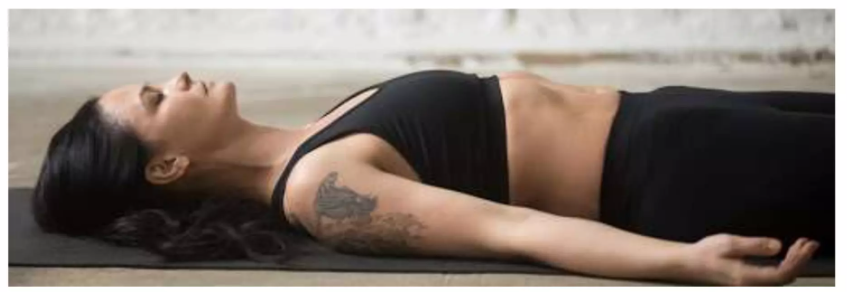
\includegraphics[width=0.8\linewidth,keepaspectratio]{yoganidra7}

		{\tiny (Ref: Yoga Nidra - Dr Amit Chail)}		
        \end{center}		
\end{frame}


%%%%%%%%%%%%%%%%%%%%%%%%%%%%%%%%%%%%%%%%%%%%%%%%%%%%%%%%%%%%%%%%%%%%%%%%%%%%%%%%%%
\begin{frame}[fragile]\frametitle{Choosing Your Sankalpa - 2}
    \begin{itemize}
        \item \textbf{Guidelines for Selection:}
        \begin{itemize}
            \item Keep it short and simple
            \item Use positive language
            \item Make it personal and meaningful
        \end{itemize}
        \item \textbf{Usage:}
        \begin{itemize}
            \item Maintain same Sankalpa across sessions
            \item Repeat until manifestation
            \item Plant during receptive state
        \end{itemize}
        \item \textbf{Examples:}
        \begin{itemize}
            \item "I am at peace with myself"
            \item "I am healthy and strong"
            \item "I am connected to my inner wisdom"
        \end{itemize}
		\item Sankalp is customized for each case, memory overwrite, e.g. pain from left foot is gone. Ideally it's a positive statement 
    \end{itemize}
\end{frame}

%%%%%%%%%%%%%%%%%%%%%%%%%%%%%%%%%%%%%%%%%%%%%%%%%%%%%%%%%%%%%%%%%%%%%%%%%%%%%%%%%%
\begin{frame}[fragile]\frametitle{Rotation of Awareness (Abbreviated) - 3}
Also called as ``Prayatna Shaithilya'' प्रयत्न शैथिल्य  as it is effortful relaxation.

\textbf{Focus on body parts:}

\begin{columns}
    \begin{column}[T]{0.3\linewidth}
    \begin{itemize}
        \item Right heel
        \item Left heel
        \item Right calf
        \item Left calf
        \item Right knee
        \item Left knee
        \item Right thigh
        \item Left thigh
        \item Both hips
        \item Lower back
        \item Upper back
        \item Right shoulder
        \item Left shoulder
        \item Back of the head
    \end{itemize}

    \end{column}
    \begin{column}[T]{0.7\linewidth}
	      \begin{center}
        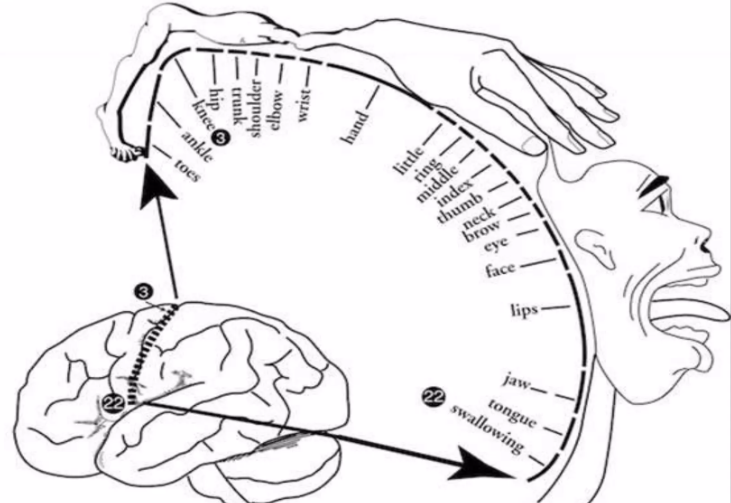
\includegraphics[width=\linewidth,keepaspectratio]{yoganidra8}

		{\tiny (Ref: Yoga Nidra - Dr Amit Chail)}		
        \end{center}
    \end{column}
  \end{columns}
	
\end{frame}

%%%%%%%%%%%%%%%%%%%%%%%%%%%%%%%%%%%%%%%%%%%%%%%%%%%%%%%%%%%%%%%%%%%%%%%%%%%%%%%%%%
\begin{frame}[fragile]\frametitle{Rotation of Awareness - Right Side}
    \begin{itemize}
        \item Begin the journey of awareness on the \textbf{right side} of the body.
        \item Focus sequentially: \textbf{Right hand} -- thumb, 2nd finger, 3rd finger, 4th finger, 5th finger, palm, back of the hand, wrist, forearm, elbow, upper arm, shoulder.
        \item Move to the \textbf{right torso and leg}: right side of chest, waist, hip, thigh, knee, calf, ankle, top of the foot, big toe, 2nd toe, 3rd toe, 4th toe, 5th toe.
    \end{itemize}
\end{frame}

%%%%%%%%%%%%%%%%%%%%%%%%%%%%%%%%%%%%%%%%%%%%%%%%%%%%%%%%%%%%%%%%%%%%%%%%%%%%%%%%%%
\begin{frame}[fragile]\frametitle{Rotation of Awareness - Left Side}
    \begin{itemize}
        \item Shift awareness to the \textbf{left side} of the body.
        \item Focus sequentially: \textbf{Left hand} -- thumb, 2nd finger, 3rd finger, 4th finger, 5th finger, palm, back of the hand, wrist, forearm, elbow, upper arm, shoulder.
        \item Move to the \textbf{left torso and leg}: left side of chest, waist, hip, thigh, knee, calf, ankle, heel, sole, top of the foot, big toe, 2nd toe, 3rd toe, 4th toe, 5th toe.
    \end{itemize}
\end{frame}

%%%%%%%%%%%%%%%%%%%%%%%%%%%%%%%%%%%%%%%%%%%%%%%%%%%%%%%%%%%%%%%%%%%%%%%%%%%%%%%%%%
\begin{frame}[fragile]\frametitle{Rotation of Awareness - Back of the Body}
    \begin{itemize}
        \item Shift awareness to the \textbf{back of the body}.
        \item Focus sequentially: soles of the feet, heels, calves, backs of knees, thighs, lower back, middle back, upper back, spine, right shoulder blade, left shoulder blade, back of the neck, back of the head, top of the head.
    \end{itemize}
\end{frame}

%%%%%%%%%%%%%%%%%%%%%%%%%%%%%%%%%%%%%%%%%%%%%%%%%%%%%%%%%%%%%%%%%%%%%%%%%%%%%%%%%%
\begin{frame}[fragile]\frametitle{Rotation of Awareness - Front of the Body}
    \begin{itemize}
        \item Shift awareness to the \textbf{front of the body}.
        \item Focus sequentially: forehead, right temple, left temple, right ear, left ear, right eyebrow, left eyebrow, space between eyebrows, right eye, left eye, right nostril, left nostril, right cheek, left cheek, upper lip, lower lip, entire mouth, chin, jaw.
        \item Move to the \textbf{throat and torso}: right collarbone, left collarbone, chest, upper abdomen, navel, lower abdomen, whole torso.
    \end{itemize}
\end{frame}

%%%%%%%%%%%%%%%%%%%%%%%%%%%%%%%%%%%%%%%%%%%%%%%%%%%%%%%%%%%%%%%%%%%%%%%%%%%%%%%%%%
\begin{frame}[fragile]\frametitle{Rotation of Awareness - Whole Body}
    \begin{itemize}
        \item \textbf{Whole Body Awareness}: Experience the entire body as a single, unified presence lying on the mat.
        \item Confirm wakefulness: Move your right toe gently, affirming, "I am awake, I am aware, and I am practicing Yoga Nidra."
    \end{itemize}
\end{frame}


%%%%%%%%%%%%%%%%%%%%%%%%%%%%%%%%%%%%%%%%%%%%%%%%%%%%%%%%%%%%%%%%%%%%%%%%%%%%%%%%%%
\begin{frame}[fragile]\frametitle{Breath Awareness Techniques - 4}
    \textbf{Progressive Breath Work:}
    \begin{itemize}
        \item Place right hand on belly, left hand on chest
        \item Observe natural breath pattern
        \item Make breath bigger gradually:
        \begin{itemize}
            \item Feel belly rise first
            \item Then chest expansion
            \item Hold briefly
            \item Release with gravity
        \end{itemize}
        \item Count breaths backwards from 27. Breathing counting is reverse just to keep us on borderline, if it was ordered we would sleep automatically.
        \item Visualize breath as golden light
		\item \textbf{Check Consciousness}: Confirm you are awake and aware by listening to the guide’s voice.
    \end{itemize}
	
So far it was mostly conscious mind level, from next step onward we will involve subconscious mind.	
\end{frame}

%%%%%%%%%%%%%%%%%%%%%%%%%%%%%%%%%%%%%%%%%%%%%%%%%%%%%%%%%%%%%%%%%%%%%%%%%%%%%%%%%%
\begin{frame}[fragile]\frametitle{Opposite Sensations (Abbreviated) - 5}
    \begin{itemize}
        \item Bring awareness to the sensation of heat
        \item Feel your whole body becoming warm.
        \item Shift awareness to cold. Feel the entire body cooling down.
        \item Release both sensations.
		\item Similarly: heaviness and lightness, pain and pleasure, love and hate, etc
    \end{itemize}
\end{frame}

%%%%%%%%%%%%%%%%%%%%%%%%%%%%%%%%%%%%%%%%%%%%%%%%%%%%%%%%%%%%%%%%%%%%%%%%%%%%%%%%%%
\begin{frame}[fragile]\frametitle{Feelings \& Sensations - Experiencing Anxiety}
    \begin{itemize}
        \item \textbf{Recall an experience of anxiety}: Feel the stress, worry, or fear without focusing on the source.
        \item Allow your body to \textbf{become aware of tension}: Notice areas of tightness or rigidity throughout the body.
    \end{itemize}
\end{frame}

%%%%%%%%%%%%%%%%%%%%%%%%%%%%%%%%%%%%%%%%%%%%%%%%%%%%%%%%%%%%%%%%%%%%%%%%%%%%%%%%%%
\begin{frame}[fragile]\frametitle{Feelings \& Sensations - Releasing Tension}
    \begin{itemize}
        \item Take a deep breath in, \textbf{visualizing relaxation} flowing into tense areas.
        \item With each inhale, feel your body becoming soft, loose, and calm.
        \item \textbf{Breathe in calmness} and exhale all stress and worries.
    \end{itemize}
\end{frame}

%%%%%%%%%%%%%%%%%%%%%%%%%%%%%%%%%%%%%%%%%%%%%%%%%%%%%%%%%%%%%%%%%%%%%%%%%%%%%%%%%%
\begin{frame}[fragile]\frametitle{Creating a Protective Space}
    \begin{itemize}
        \item \textbf{Visualize your IshtaDevata} (favorite deity, teacher, or higher consciousness) sending positive energy.
        \item Imagine a circle of protection around you, creating a \textbf{safe and peaceful space}.
        \item Feel calm, safe, and secure in this protected space.
    \end{itemize}
\end{frame}

%%%%%%%%%%%%%%%%%%%%%%%%%%%%%%%%%%%%%%%%%%%%%%%%%%%%%%%%%%%%%%%%%%%%%%%%%%%%%%%%%%
\begin{frame}[fragile]\frametitle{Revisiting Anxiety in a Safe Space}
    \begin{itemize}
        \item While feeling secure, \textbf{recall the experience of anxiety}, observing it without attachment.
        \item Notice how the anxiety melts away, protected by the presence of your IshtaDevata.
        \item This space is \textbf{free from worries and tension}; it is your safe and peaceful zone.
    \end{itemize}
\end{frame}

%%%%%%%%%%%%%%%%%%%%%%%%%%%%%%%%%%%%%%%%%%%%%%%%%%%%%%%%%%%%%%%%%%%%%%%%%%%%%%%%%%
\begin{frame}[fragile]\frametitle{Affirmation of Peace}
    \begin{itemize}
        \item Remain in this space, breathing deeply, visualizing all \textbf{tension and worries floating away}.
        \item Repeat to yourself: \textit{"I am calm, peaceful, and free from anxiety."}
        \item Believe in this affirmation with faith and conviction.
    \end{itemize}
\end{frame}


%%%%%%%%%%%%%%%%%%%%%%%%%%%%%%%%%%%%%%%%%%%%%%%%%%%%%%%%%%%%%%%%%%%%%%%%%%%%%%%%%%
\begin{frame}[fragile]\frametitle{Guided Imagery (Abbreviated) - 6}
    \textbf{Journey through Nature:}
    \begin{itemize}
        \item Imagine standing in a meadow, surrounded by a lush forest.
        \item Feel the warmth of the sun and smell the wildflowers.
        \item Walk into the forest, following a path that leads uphill.
        \item Reach a cave and discover a lit candle inside.
        \item Meditate on the candle's flame, with your Sankalpa inscribed on it.
    \end{itemize}
	
Visualization is 5-6 minutes long to impart something in the memory. Here also customization can be done.
	
\end{frame}

%%%%%%%%%%%%%%%%%%%%%%%%%%%%%%%%%%%%%%%%%%%%%%%%%%%%%%%%%%%%%%%%%%%%%%%%%%%%%%%%%%
\begin{frame}[fragile]\frametitle{Visualization (Symbols)}
    \begin{itemize}
        \item \textbf{Instructions}: Visualize each image briefly, allowing it to resonate with your emotions, memories, or imagination.
        \item \textbf{Jump from image to image} without lingering.
    \end{itemize}
    \vspace{0.5cm}
    \begin{columns}
        \column{0.5\textwidth}
            \begin{itemize}
                \item Cool Clear Water
                \item Vibrant Sunset
                \item Tall mountains
                \item Traffic Lights
                \item A good night’s rest
                \item Deep Breath
                \item Beautiful Garden
                \item Temple Bells Ringing
                \item Deep Blue Sky
                \item Relaxing afternoon
            \end{itemize}
        \column{0.5\textwidth}
            \begin{itemize}
                \item A cat stretching
                \item A warm hug
                \item Doctor's office
                \item Your reflection in a mirror
                \item Meditating Buddha
                \item Mother
                \item Ancestral Home
                \item Laughing with friends
                \item The sound of my voice
                \item Your body lying on the floor
            \end{itemize}
    \end{columns}
\end{frame}

%%%%%%%%%%%%%%%%%%%%%%%%%%%%%%%%%%%%%%%%%%%%%%%%%%%%%%%%%%%%%%%%%%%%%%%%%%%%%%%%%%
\begin{frame}[fragile]\frametitle{Sankalpa - 7}
    \begin{itemize}
        \item \textbf{Repeat your Sankalpa} three times with focus, clarity, and determination.
        \item Visualize your sankalpa taking shape and becoming successful.
        \item Feel your sankalpa bearing fruit and manifesting in your life.
    \end{itemize}
\end{frame}

%%%%%%%%%%%%%%%%%%%%%%%%%%%%%%%%%%%%%%%%%%%%%%%%%%%%%%%%%%%%%%%%%%%%%%%%%%%%%%%%%%
\begin{frame}[fragile]\frametitle{Exiting the Practice}
    \begin{itemize}
        \item Gradually bring awareness back to your breath, feeling it flow in and out of your nostrils.
        \item Shift awareness to your physical body lying on the floor, noticing all points of contact.
        \item \textbf{Awareness of Sounds}:
            \begin{itemize}
                \item Sounds within the room, around your mat, and the sound of my voice.
                \item Expand awareness to sounds outside the room.
            \end{itemize}
        \item Visualize the room and your position within it.
        \item Slowly begin to move: 
            \begin{itemize}
                \item Move hands and feet gently.
                \item Roll over to the right side, revisiting feelings of safety, calm, and peace.
                \item Use your left hand to sit up comfortably.
            \end{itemize}
        \item Take a deep breath, exhale fully. Rub palms to create warmth and place them over your eyes.
        \item Open your eyes gently, and blink your eyes open while looking into your palms.
    \end{itemize}
    \vspace{0.5cm}
    \textbf{The practice of Yoga Nidra is now complete.}
\end{frame}

%%%%%%%%%%%%%%%%%%%%%%%%%%%%%%%%%%%%%%%%%%%%%%%%%%%%%%%%%%%%%%%%%%%%%%%%%%%%%%%%%%
\begin{frame}[fragile]\frametitle{Post-Practice Reflection}
    \textbf{Journaling Guidelines:}
    \begin{itemize}
        \item Record your experience immediately after practice
        \item Note any physical sensations experienced
        \item Document emotional states encountered
        \item Track progress over time
        \item Record any insights or revelations
        \item Compare experiences across different sessions
    \end{itemize}
    \small{This reflection helps deepen your practice and track your progress.}
\end{frame}

%%%%%%%%%%%%%%%%%%%%%%%%%%%%%%%%%%%%%%%%%%%%%%%%%%%%%%%%%%%%%%%%%%%%%%%%%%%%%%%%%%
\begin{frame}[fragile]\frametitle{Best Practices for Teachers}
    \begin{itemize}
        \item \textbf{Voice and Delivery:}
        \begin{itemize}
            \item Speak in a soothing, even tone
            \item Maintain consistent pace
            \item Use clear, simple language
            \item Allow adequate pauses
        \end{itemize}
        \item \textbf{Session Management:}
        \begin{itemize}
            \item Start with shorter sessions (20-30 minutes)
            \item Progress gradually to longer sessions
            \item Always complete all stages
            \item Monitor student comfort
        \end{itemize}
    \end{itemize}
\end{frame}

%%%%%%%%%%%%%%%%%%%%%%%%%%%%%%%%%%%%%%%%%%%%%%%%%%%%%%%%%%%%%%%%%%%%%%%%%%%%%%%%%%
\begin{frame}[fragile]\frametitle{Children's Practice Considerations}
    \begin{itemize}
        \item \textbf{Session Duration:}
        \begin{itemize}
            \item Keep sessions shorter (10-15 minutes)
            \item Use age-appropriate language
            \item Include playful visualization
        \end{itemize}
        \item \textbf{Special Elements:}
        \begin{itemize}
            \item Use simple counting exercises (40 to 1)
            \item Include light visualization exercises
            \item Incorporate gentle encouragement
            \item Allow natural breaks in concentration
        \end{itemize}
        \item \textbf{Closing Practice:}
        \begin{itemize}
            \item End with positive affirmations
            \item Include sharing of "light" with loved ones
            \item Gentle return to regular awareness
        \end{itemize}
    \end{itemize}
\end{frame}